\documentclass{uninove-ppgi} %courier ou times

\begin{document}
\lstset{
    language=xml,
    tabsize=3,
    frame=shadowbox,
    rulesepcolor=\color{gray},
    xleftmargin=20pt,
    framexleftmargin=15pt,
    keywordstyle=\color{blue}\bf,
    commentstyle=\color{OliveGreen},
    stringstyle=\color{red},
    numbers=left,
    numberstyle=\tiny,
    numbersep=5pt,
    breaklines=true,
    showstringspaces=false,
    basicstyle=\footnotesize,
    emph={food,name,price},emphstyle={\color{magenta}}
}

% Posiciona o logo da Uni9 no topo
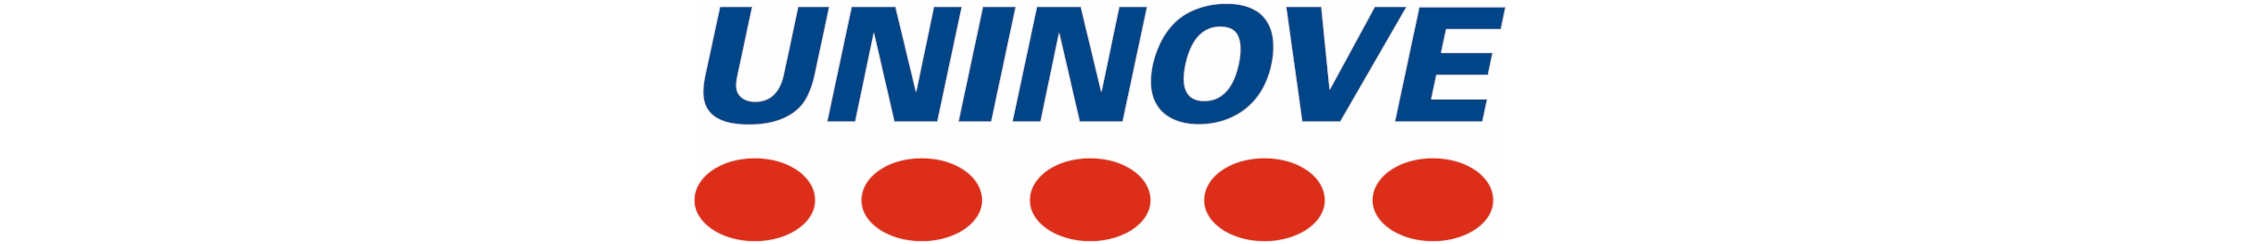
\includegraphics[height=1.5cm]{uninove-logo}

% parametros de capa e folha de rosto (é necessário configurar todos)
\Universidade{UNIVERSIDADE NOVE DE JULHO - UNINOVE}

\Autor{EXCLUÍDOS OS DADOS SOBRE OS AUTORES EM ATENDIMENTO A LGPD - LEI GERAL DE PROTEÇÃO DE DADOS}

% ATENÇÃO: NÃO INCLUIR NOME E RA DE NENHUM ALUNO
% EM NENHUMA PARTE DO DOCUMENTO

\Titulo{CUBO DE RUBIK}

% Inserir o nome do projeto no formato que está abaixo (Olhe o nome da disciplina na central do aluno)
\Tipoprojeto{NOME DO PROJETO EM COMPUTAÇÃO APLICADA}

% Informe qual o curso: Bacharel ou Tecnólogo + curso
\Curso{Bacharel em Ciência da Computação}

% NÃO ALTERAR
\Orientador{Edson Melo de Souza, Dr.}

% Inserir o ano correspondente
\Ano{2024}

% gera a capa automaticamente
\capa

% gera folha de rosto automaticamente
\folharosto

% ##################### Início dos elementos pré-textuais ############################

% Resumo (Obrigatório)
\input{pre_textuais/04_resumo.tex}

% Abstract (Obrigatório) - resumo em inglês
\input{pre_textuais/05_abstract.tex}

% Sumário (Obrigatório)
\begingroup
\makeatletter \let\ps@plain\ps@empty \makeatother
\tableofcontents % sumário
\endgroup
\thispagestyle{empty}

% Lista de figuras
\renewcommand*\listfigurename{Lista de Ilustrações}
\listoffigures
\thispagestyle{empty}

% ############### Fim dos elementos pré-textuais ######################

\regularchapterstyle

% ############### Início dos Capítulos (Obrigatório ) #################

% Introdução
\input{capitulos/cap01_introducao.tex}

% Interface da aplicação
\input{capitulos/cap02_interface_da_aplicacao.tex}

% Botão visualizar
\input{capitulos/cap03_botao_visualizar.tex}

% Botão criptografar
\input{capitulos/cap04_botao_criptografar.tex}

% Botão descriptografar
\input{capitulos/cap05_botao_descriptografar.tex}

% Botão real
\input{capitulos/cap06_botao_tempo_real.tex}

% Botão arquivo e gerar arquivo
\input{capitulos/cap07_arquivo.tex}

% Botão de criptografar e desciptografar o arquivo de texto
\input{capitulos/cap08_crip_descrip_arq.tex}

% Conclusão
\input{capitulos/cap09_conclusao.tex}

% ##################### Fim dos Capítulos ############################

% Bibliografia (Obrigatório)
\bibliography{refs}
    \begin{enumerate}
            \item Leitura e salvamento do arquivo: \href{https://learn.microsoft.com/pt-br/troubleshoot/developer/visualstudio/csharp/language-compilers/read-write-text-file}{https://learn.microsoft.com/pt-br/troubleshoot/
            developer/visualstudio/csharp/language-compilers/read-write-text-file}

            \item Sobre tipos de criptografia e sua importância: \href{https://shorturl.at/dquY9}
            {https://shorturl.at/dquY9}

            \item Inspiração para o método de criptografia: \href{https://pt.wikipedia.org/wiki/Cifra_de_César}
            {https://pt.wikipedia.org/wiki/Cifra-de-César}

            \item Código de pesquisa por pastas: \href{https://youtu.be/PP5QkpUDak0?feature=shared }
            {https://youtu.be/PP5QkpUDak0?feature=shared}
    \end{enumerate}

\end{document}